\cleardoublepage


\chapter{Direkte Kinematik}

Die direkte Kinematik ist dafür verantwortlich aus den verschiedenen Winkeln und Positionen der Gelenke die Rotation und Position des Endeffektors im Raum zu berechnen.
Dazu wird zunächst in jedem Gelenk ein Koordinatenursprung gelegt, der eine Nullstellung jedes Gelenks beschreibt.
Um alle Gelenke in einer kinematischen Kette abzubilden, kann dann beispielsweise mithilfe der homogenen Transformationsmatrix (Abschnitt~\ref{sec:homogene-transformationsmatrix}) und einem Parameter in den Freiheitsgraden des entsprechenden Gelenks eine Rechenvorschrift aufgebaut werden, um den Roboter zu beschreiben und die Position des Endeffektors schnell bestimmen zu können. (?? Quelle)


\section{DH-Konvention}

(?? Quelle)

Die Konvention, die in der Regel verwendet wird, um Rotation und Translation eines Gliedes der kinematischen Kette darzustellen ist die sog.\ \ac{dhk} oder DH-Transformation.
\ac{dhk} beschreibt, wie die Koordinatensysteme basieren auf dem vorherigen Koordinatensystem beschrieben werden.
Um nun ausgehend von Gelenk $n-1$ das Koordinatensystem von Gelenk $n$ zu beschreiben, müssen die folgenden Regeln befolgt werden:

\begin{enumerate}
    \item Achse $z_{n}$ liegt entlang der Bewegungsachse von Gelenk des Gelenks
    \item Achse $x_{n}$ liegt auf der kürzesten Verbindung zwischen Achsen $z{n-1}$ und $z_{n}$.
    \item Die $y_{n}$ Achse wird rechtshändig ergänzt.
\end{enumerate}

Dabei sind die Ursprünge der Gelenkkordinatensysteme oftmals nicht im Gelenkursprung, was Komplexität für die Berechnung von Transformationen verringert.
Aus der Beziehung der zwei Koordinatensysteme können die DH-Parameter abgeleitet werden (siehe auch Abbildung~\ref{fig:dh-konvention1}):

\begin{itemize}
    \item $\theta_n$ Winkel zwischen $x_{n-1}$ und $x_n$ mit Rotationsachse $z_{n-1}$
    \item $d_n$: Kleinster Abstand zwischen $x_{n-1}$ und $x_n$
    \item $a_n$: Abstand zwischen den Achsen $z_{n-1}$ und $z_n$
    \item $\alpha_n$ Winkel zwischen $z_{n-1}$ und $z_n$ mit Rotationsachse $x_{n}$
\end{itemize}

Dies entspricht den folgenden Transformationsmatrizen (Gleichungen~\ref{eq:dh1},~\ref{eq:dh2},~\ref{eq:dh3},~\ref{eq:dh4}):

\newcommand{\ct}{\cos(\theta_n)}
\newcommand{\st}{\sin(\theta_n)}
\newcommand{\ca}{\cos(\alpha_n)}
\newcommand{\sa}{\sin(\alpha_n)}

\begin{equation}
    \[
        T_{\theta_n} =
        \left[ {\begin{array}{cccc}
                    \ct & -\st & 0 & 0 \\
                    \st & \ct  & 0 & 0 \\
                    0   & 0    & 1 & 0 \\
                    0   & 0    & 0 & 1 \\
        \end{array} } \right]
    \]\label{eq:dh1}
\end{equation}

\begin{equation}
    \[
        T_{d_n} =
        \left[ {\begin{array}{cccc}
                    1 & 0 & 0 & 0   \\
                    0 & 1 & 0 & 0   \\
                    0 & 0 & 1 & d_n \\
                    0 & 0 & 0 & 1   \\
        \end{array} } \right]
    \]\label{eq:dh2}
\end{equation}

\begin{equation}
    \[
        T_{a_n} =
        \left[ {\begin{array}{cccc}
                    1 & 0 & 0 & a_n \\
                    0 & 1 & 0 & 0   \\
                    0 & 0 & 1 & 0   \\
                    0 & 0 & 0 & 1   \\
        \end{array} } \right]
    \]\label{eq:dh3}
\end{equation}

\begin{equation}
    \[
        T_{\alpha_n} =
        \left[ {\begin{array}{cccc}
                    1 & 0   & 0    & 0 \\
                    0 & \ca & -\sa & 0 \\
                    0 & \sa & \ca  & 0 \\
                    0 & 0   & 0    & 1 \\
        \end{array} } \right]
    \]\label{eq:dh4}
\end{equation}

Um nun Koordinatensystem $n-1$ in Koordinatensystem $n$ zu überführen, kann die Transformationsmatrix $T_{n-1,n}$ verwendet werden (Gleichung~\ref{eq:dh5}).

\begin{equation}
    \[
        T_{n-1,n} = T_{\theta_n} \cdot T_{d_n} \cdot T_{a_n} \cdot T_{\alpha_n} =
        \left[ {\begin{array}{cccc}
                    \ct & -\st\ca & \st\sa & a_n\ct \\
                    \st & \ct\ca  & -ct\sa & a_n\st \\
                    0   & \sa     & \ca    & d_n    \\
                    0   & 0       & 0      & 1      \\
        \end{array} } \right]
    \]\label{eq:dh5}
\end{equation}

\begin{figure}[h]
    \centering
    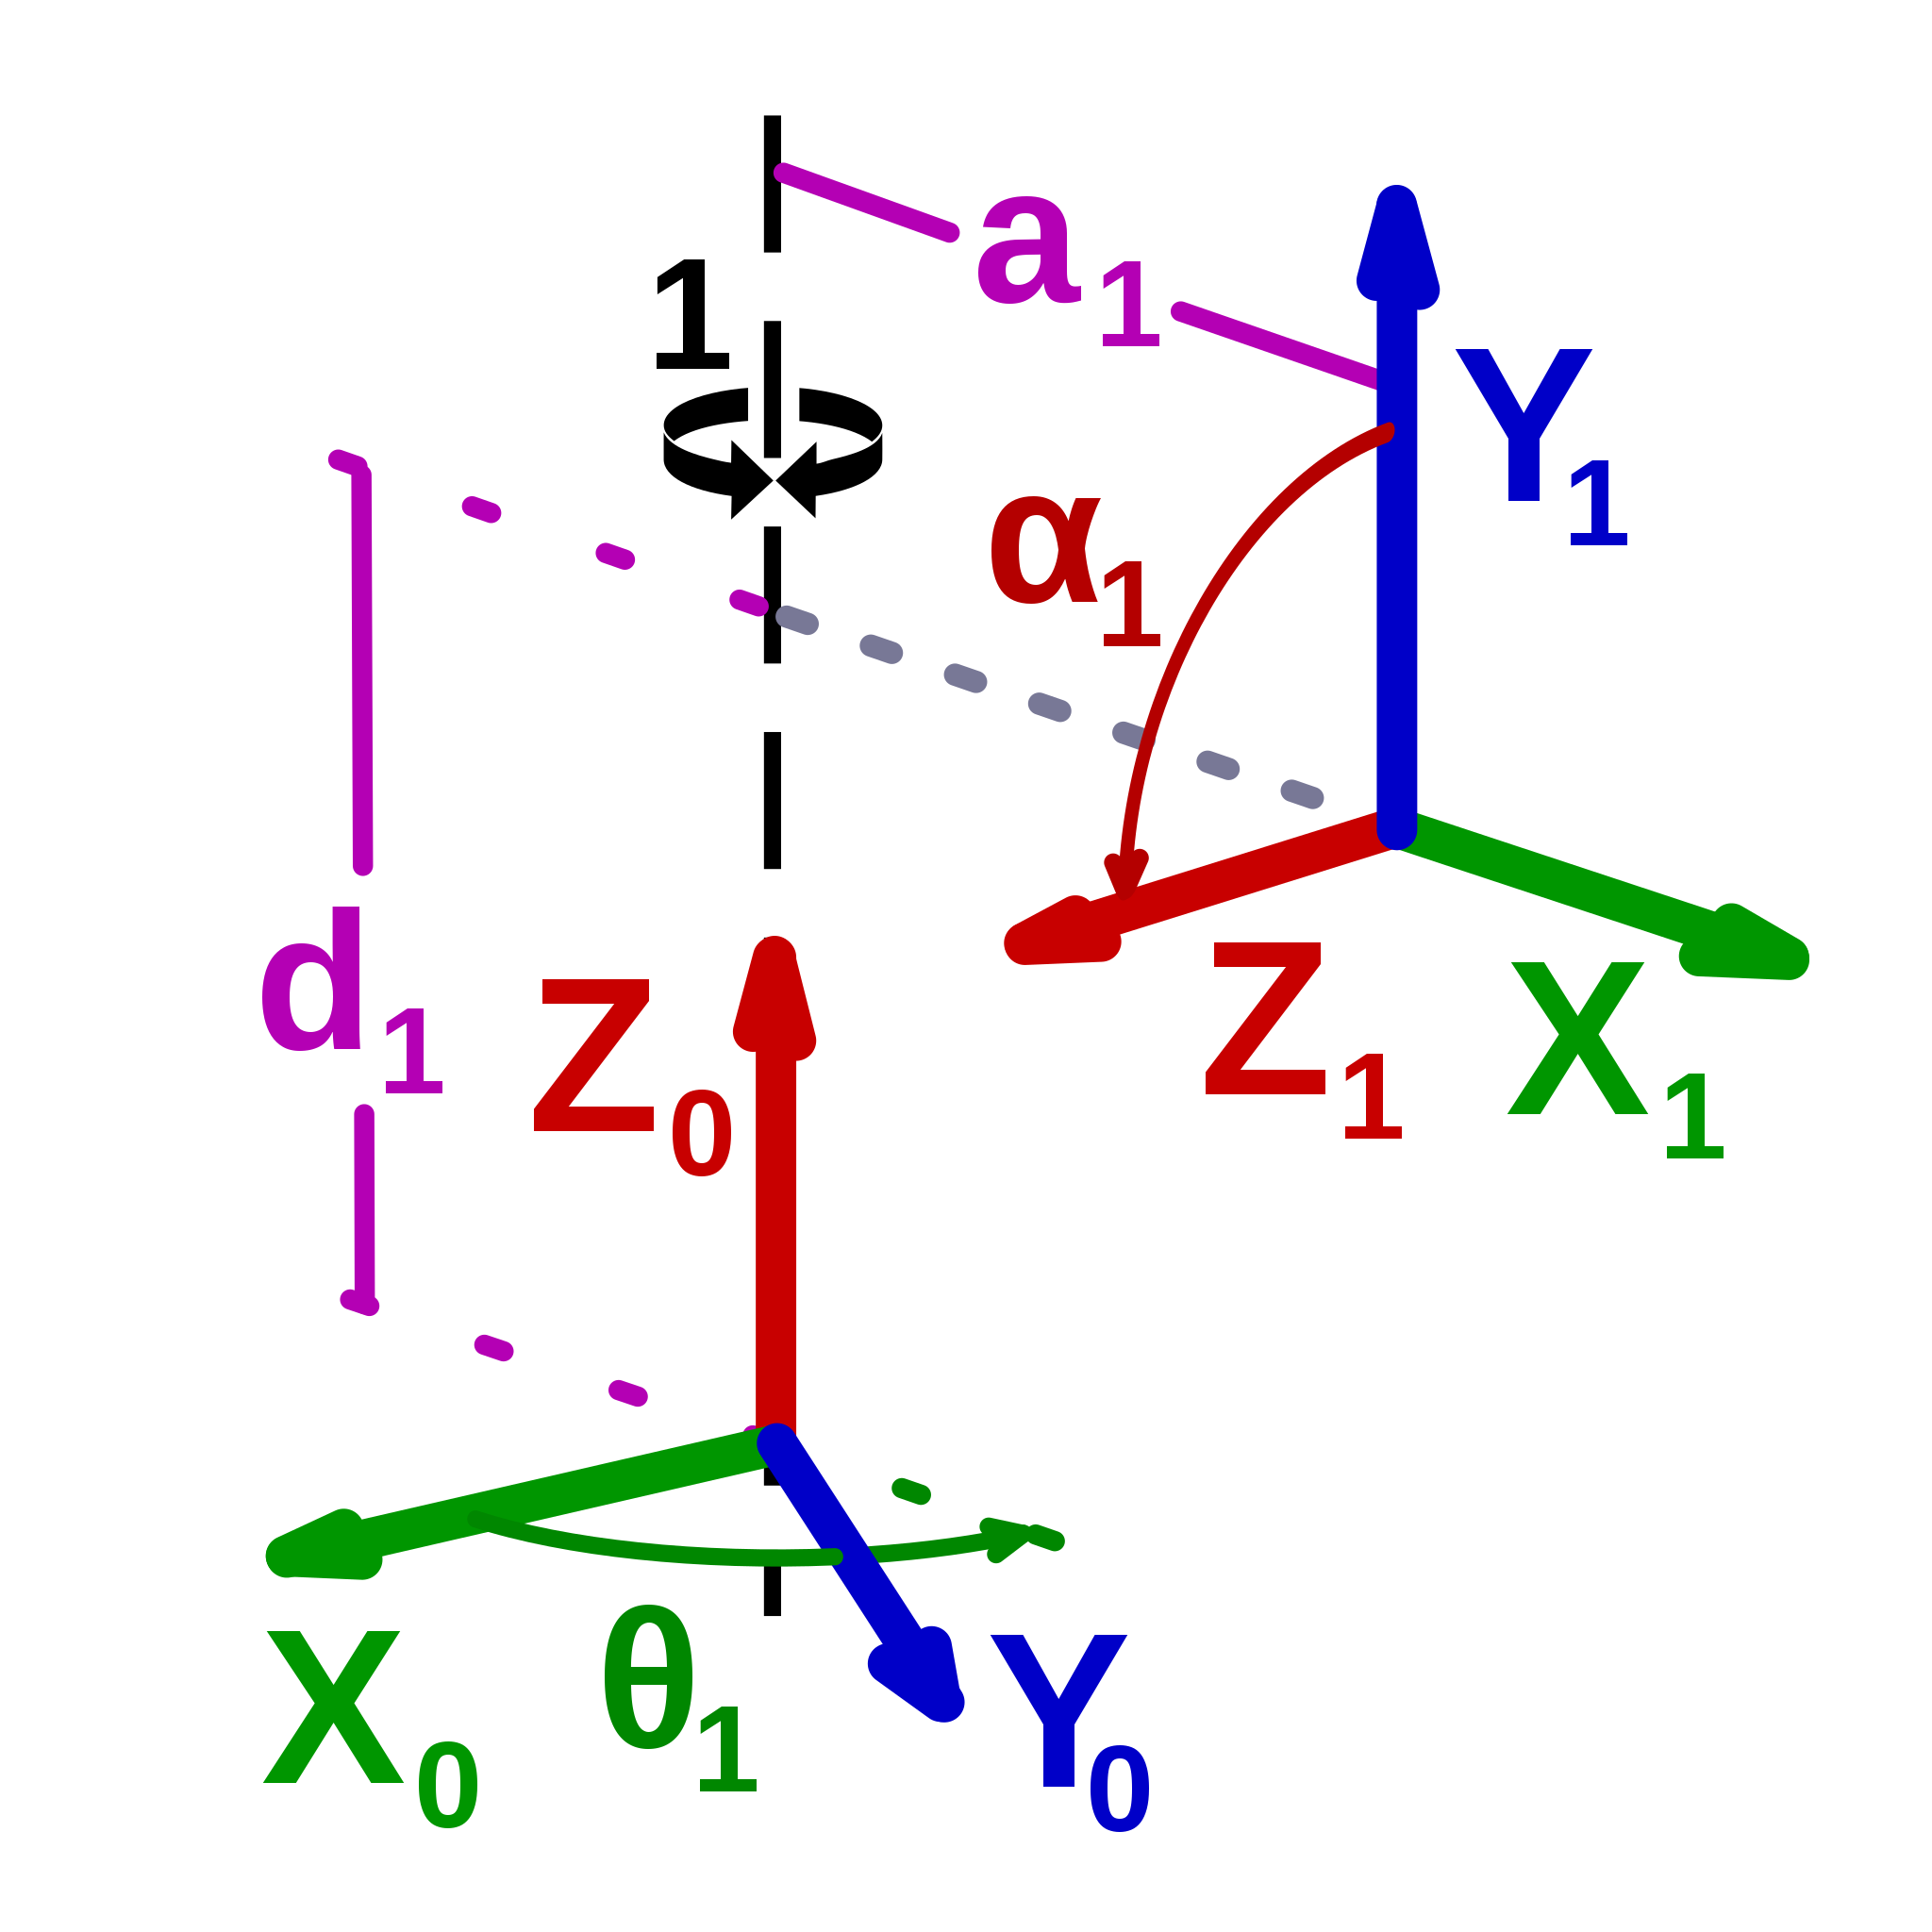
\includegraphics[width = .5\textwidth]{Bilder/Denavit-Hartenberg-Transformation.svg}
    \caption{\ac{dhk} zwischen zwei Gelenken ?? https://de.wikipedia.org/wiki/Datei:Denavit-Hartenberg-Transformation.svg}\label{fig:dh-konvention1}
\end{figure}


\section{URDF}


\section{Robotics API}


\section{UR5 in DH}

